\section{Experimentation}
\label{sec:experimentation}
\subsection{First experiment}
The goal of the first experiment is to observe the differences of applying EM and DBSCAN to the generated data with blob shape. For this, we created an algorithm that given a number of blobs ($n_b$) and the space between them ($s_b$), it places the $n_b$ isotropic Gaussian blobs in a well-distributed way, and with centers separated at a distance of $s_b$ (see table \ref{tab:data-param}). We tried EM and DBSCAN for several cases generated with the algorithm, but we selected 4 of them that show clearly the differences between both. %which are represented in sub-figures \ref{subfig:4-4-truth}, \ref{subfig:7-3-truth}, \ref{subfig:30-30-truth} and \ref{subfig:30-30-6-truth}.
\begin{table}[hbtp]
    \centering
    \begin{tabular}{c c c}
        \toprule
        \textbf{Sub-figure} & $\bm{n_b}$ & $\bm{s_b}$ \\ \midrule
        \ref{subfig:4-4-truth} & 4 & 2 \\
        \ref{subfig:7-3-truth} & 7 & 2 \\
        \ref{subfig:30-30-truth} & 30 & 2 \\
        \ref{subfig:30-30-6-truth} & 30 & 6 \\
        \bottomrule
    \end{tabular}
    \caption{Parameters for the generation of the the blob shape data}
    \label{tab:data-param}
\end{table}

The selected parameters for EM ($k$) vary for each dataset, but for DBSCAN we fixed them to $\varepsilon = 0.2$ and $minPts = 10$, with which we obtained better results after trying several possibilities. Next, we explain the results of this experiment.
\begin{itemize}
    \item \textbf{4 blobs.}
\end{itemize}
\begin{figure*}[t!]
    \begin{subfigure}[b]{0.45\textwidth}
            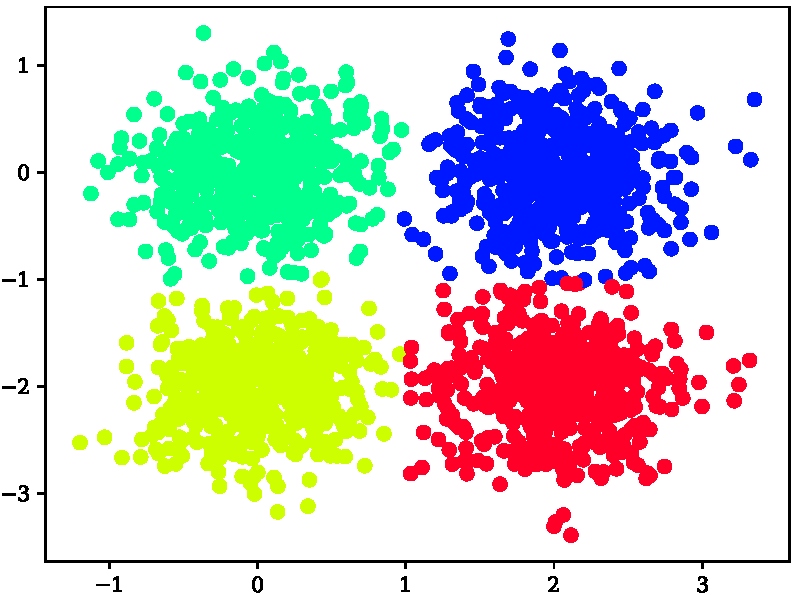
\includegraphics[width=\textwidth]{../plots/4-4_pred_em.pdf}
            \caption{EM $k = 4$}
            \label{subfig:4-4-em}
    \end{subfigure}
    \hspace{0.09\textwidth}
    \begin{subfigure}[b]{0.45\textwidth}
        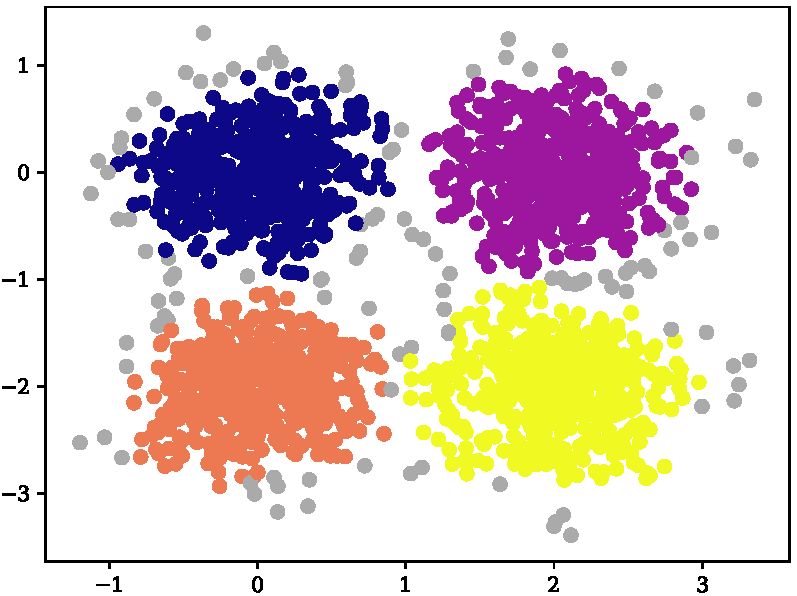
\includegraphics[width=\textwidth]{../plots/4-4_pred_dbscan.pdf}
        \caption{DBSCAN}
        \label{subfig:4-4-dbscan}
    \end{subfigure}
    \begin{subfigure}[b]{0.45\textwidth}
        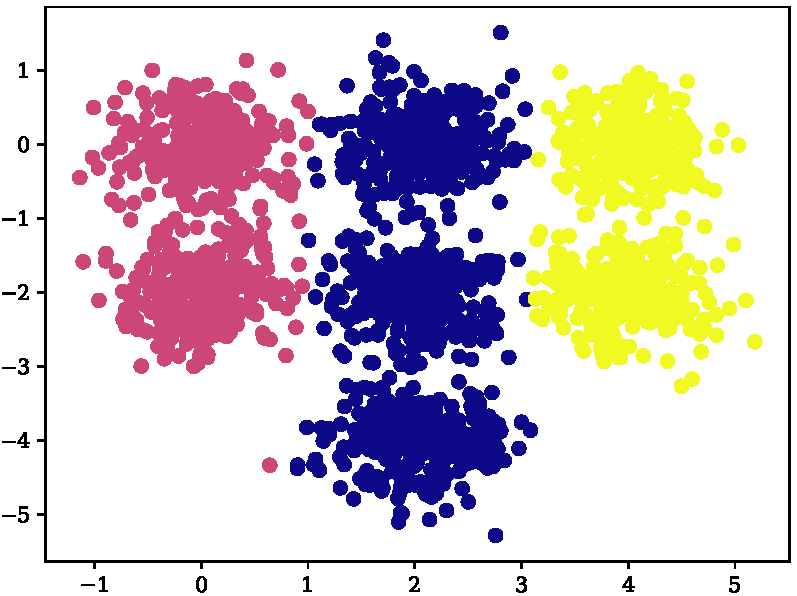
\includegraphics[width=\textwidth]{../plots/7-3_pred_em.pdf}
        \caption{EM $k = 3$}
        \label{subfig:7-3-em}
    \end{subfigure}
    \hspace{0.09\textwidth}
    \begin{subfigure}[b]{0.45\textwidth}
        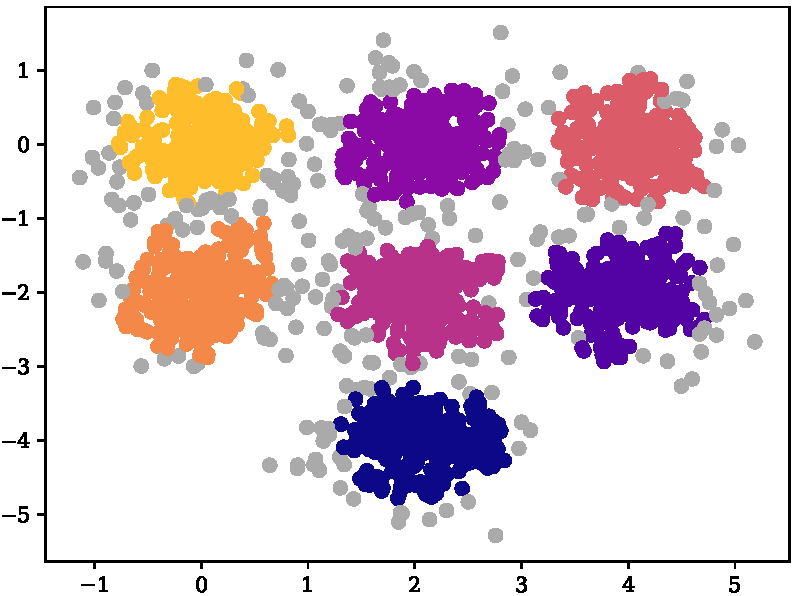
\includegraphics[width=\textwidth]{../plots/7-3_pred_dbscan.pdf}
        \caption{DBSCAN}
        \label{subfig:7-3-dbscan}
    \end{subfigure}
    \begin{subfigure}[b]{0.45\textwidth}
        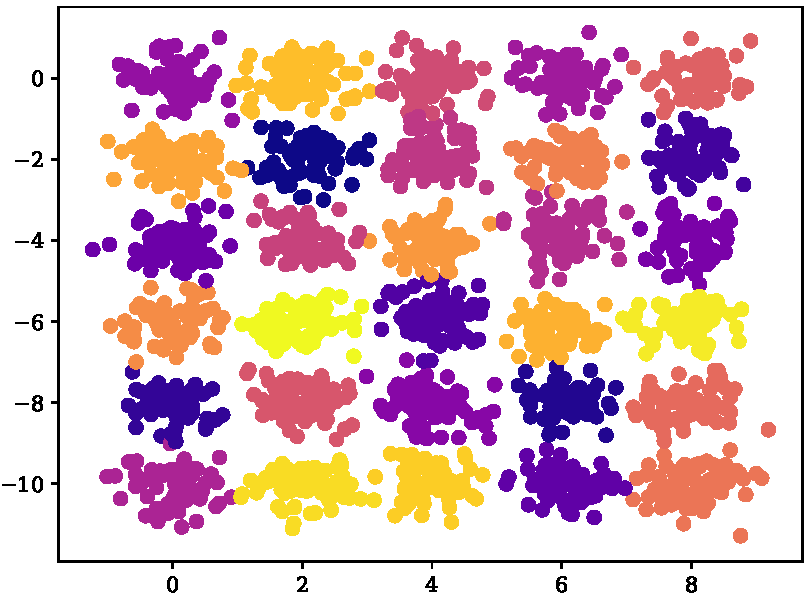
\includegraphics[width=\textwidth]{../plots/30-30_pred_em.pdf}
        \caption{EM $k = 30$}
        \label{subfig:30-30-em}
    \end{subfigure}
    \hspace{0.09\textwidth}
    \begin{subfigure}[b]{0.45\textwidth}
        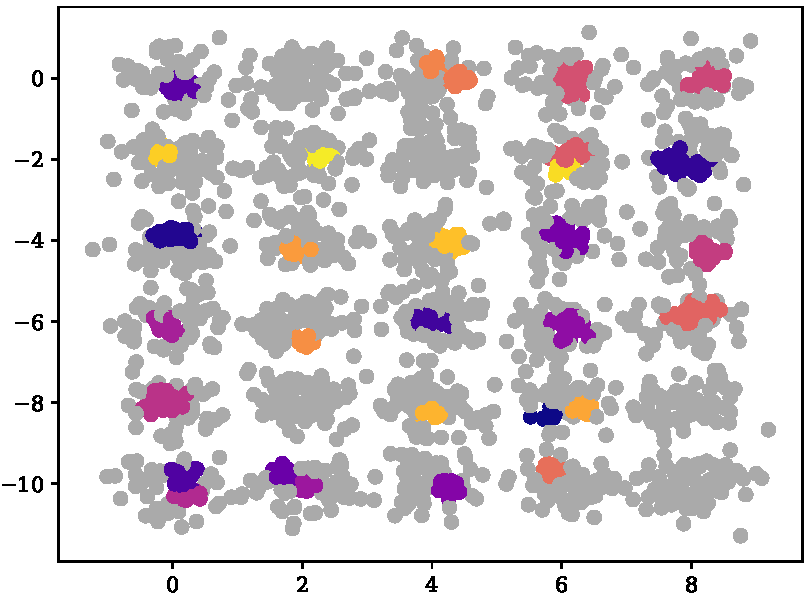
\includegraphics[width=\textwidth]{../plots/30-30_pred_dbscan.pdf}
        \caption{DBSCAN}
        \label{subfig:30-30-dbscan}
    \end{subfigure}
\end{figure*}
\begin{figure*}[t!]
    \begin{subfigure}[b]{0.45\textwidth}
        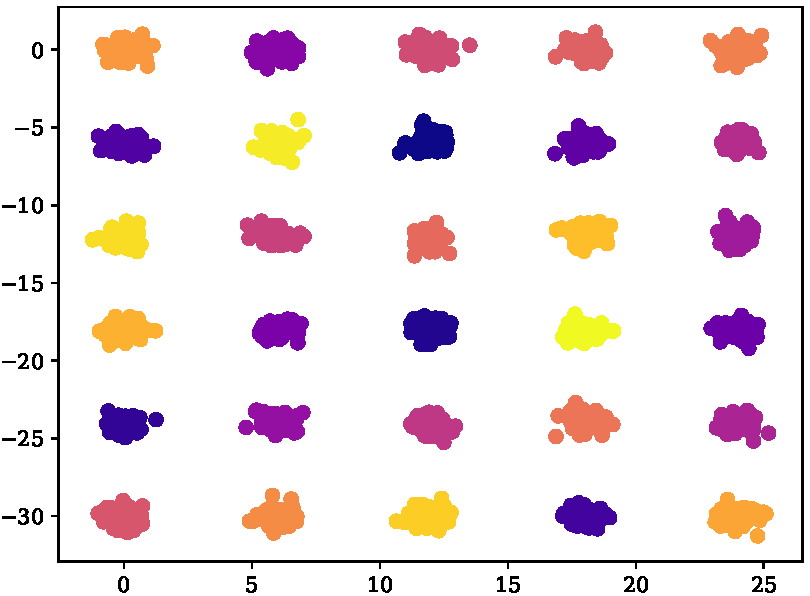
\includegraphics[width=\textwidth]{../plots/30-30-6_pred_em.pdf}
        \caption{EM $k = 30$}
        \label{subfig:30-30-6-em}
    \end{subfigure}
    \hspace{0.09\textwidth}
    \begin{subfigure}[b]{0.45\textwidth}
        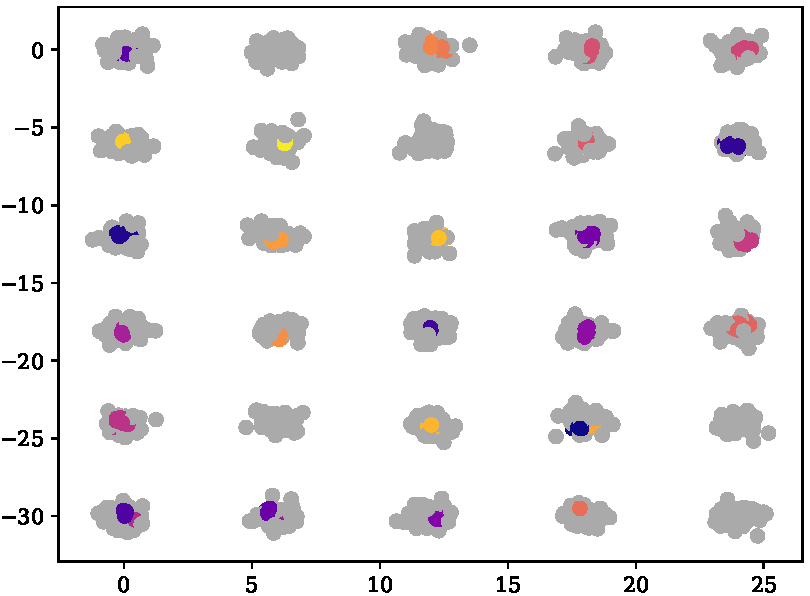
\includegraphics[width=\textwidth]{../plots/30-30-6_pred_dbscan.pdf}
        \caption{DBSCAN}
        \label{subfig:30-30-6-dbscan}
    \end{subfigure}
    \begin{subfigure}[b]{0.45\textwidth}
        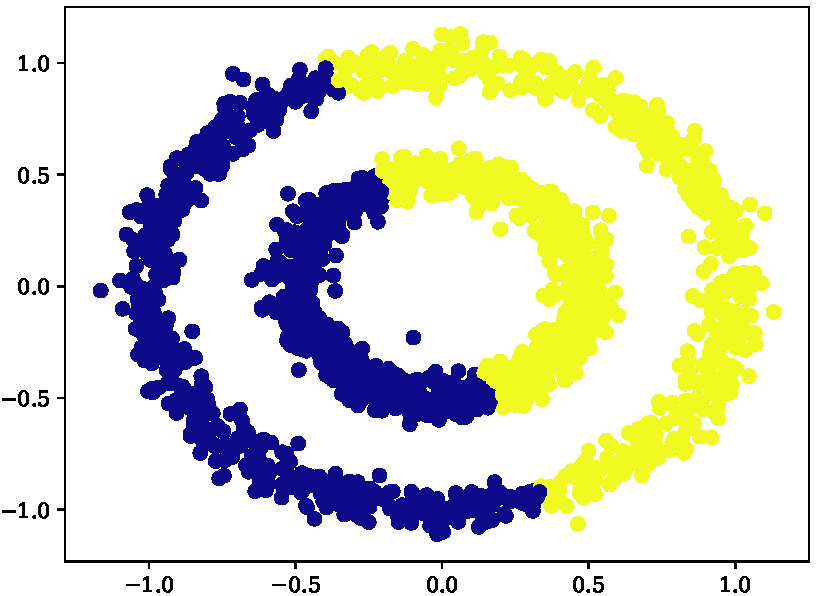
\includegraphics[width=\textwidth]{../plots/circle_em.pdf}
        \caption{EM $k = 2$}
        \label{subfig:circle-em}
    \end{subfigure}
    \hspace{0.09\textwidth}
    \begin{subfigure}[b]{0.45\textwidth}
        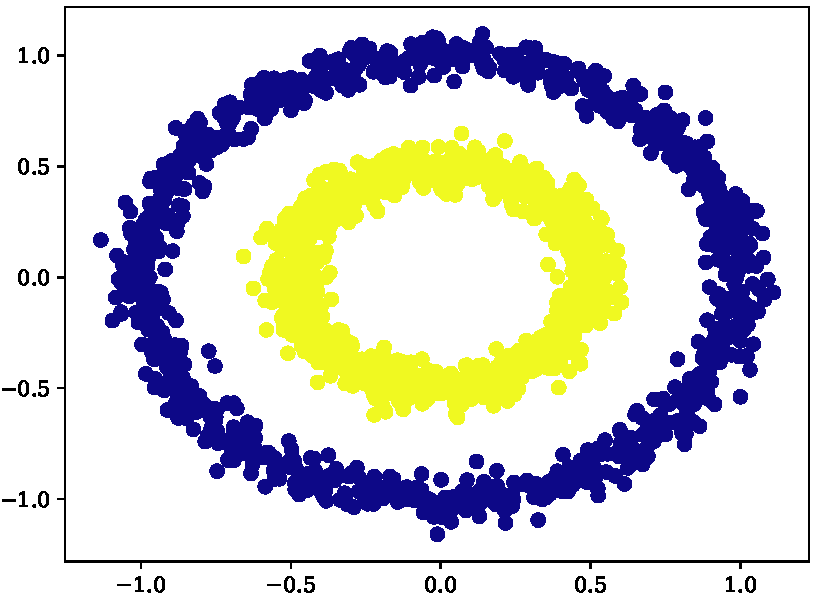
\includegraphics[width=\textwidth]{../plots/circle_dbscan.pdf}
        \caption{DBSCAN}
        \label{subfig:circle-dbscan}
    \end{subfigure}
    \begin{subfigure}[b]{0.45\textwidth}
        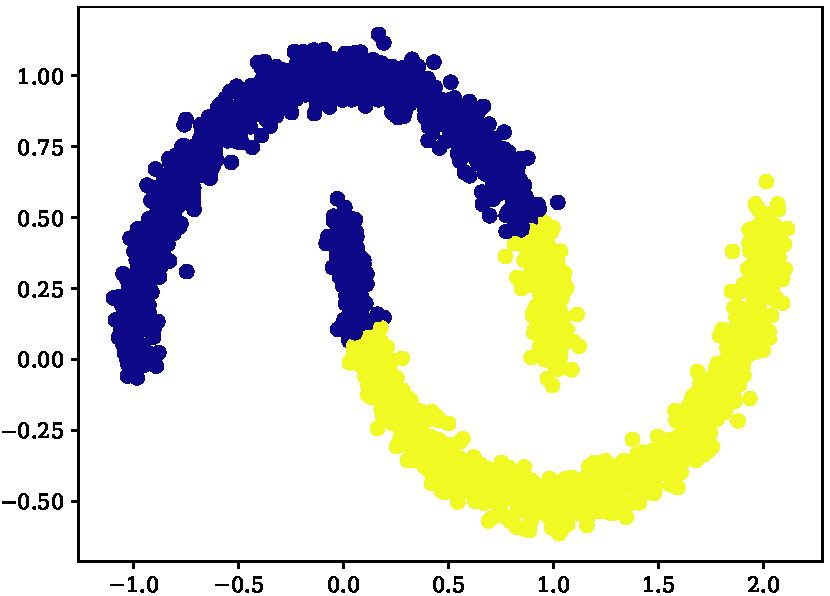
\includegraphics[width=\textwidth]{../plots/moons_em.pdf}
        \caption{EM $k = 2$}
        \label{subfig:moon-em}
    \end{subfigure}
    \hspace{0.09\textwidth}
    \begin{subfigure}[b]{0.45\textwidth}
        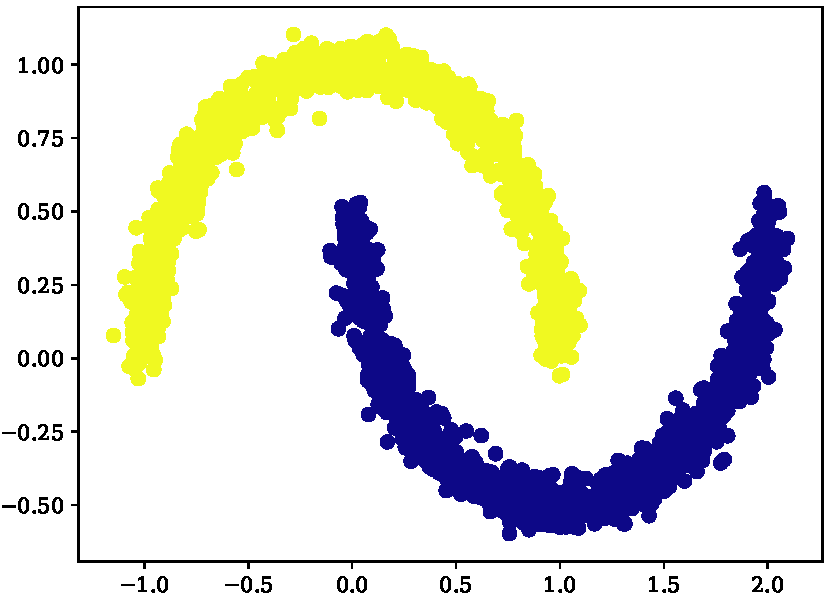
\includegraphics[width=\textwidth]{../plots/moons_dbscan.pdf}
        \caption{DBSCAN}
        \label{subfig:moon-dbscan}
    \end{subfigure}
\end{figure*}
